% Two-column technical article (working-paper edition). Every result is a macro from numbers.tex or a table from
% tables/, written by code/06_paper_numbers.py from output/*.json. Build: pdflatex inspection_rd_article (twice).
\documentclass[10pt,twocolumn,letterpaper]{article}
\usepackage[T1]{fontenc}
\usepackage[utf8]{inputenc}
\usepackage{utopia}
\usepackage[letterpaper,left=0.68in,right=0.68in,top=0.85in,bottom=0.9in,columnsep=0.22in,headsep=0.3in]{geometry}
\usepackage{amsmath,amssymb}
\usepackage{graphicx,booktabs,array,multirow,enumitem,xcolor,url}
\usepackage[font=footnotesize]{caption}
\usepackage{titlesec,fancyhdr,microtype,cite,stfloats}
\usepackage[hidelinks]{hyperref}
\newcommand{\absentLater}{87}
\newcommand{\balMonthEighty}{+0.13}
\newcommand{\balMonthNinety}{+0.06}
\newcommand{\balMonthPEighty}{0.31}
\newcommand{\balMonthPNinety}{0.58}
\newcommand{\balMonthSeEighty}{0.13}
\newcommand{\balMonthSeNinety}{0.11}
\newcommand{\balPrevEighty}{$-$0.63}
\newcommand{\balPrevNinety}{+0.57}
\newcommand{\balPrevPEighty}{0.38}
\newcommand{\balPrevPNinety}{0.35}
\newcommand{\balPrevSeEighty}{0.72}
\newcommand{\balPrevSeNinety}{0.61}
\newcommand{\balSeqEighty}{$-$0.04}
\newcommand{\balSeqNinety}{$-$0.01}
\newcommand{\balSeqPEighty}{0.33}
\newcommand{\balSeqPNinety}{0.83}
\newcommand{\balSeqSeEighty}{0.04}
\newcommand{\balSeqSeNinety}{0.03}
\newcommand{\balYearEighty}{$-$0.03}
\newcommand{\balYearNinety}{+0.04}
\newcommand{\balYearPEighty}{0.64}
\newcommand{\balYearPNinety}{0.39}
\newcommand{\balYearSeEighty}{0.05}
\newcommand{\balYearSeNinety}{0.05}
\newcommand{\ciHiEighty}{0.47}
\newcommand{\ciHiNinety}{0.56}
\newcommand{\ciLoEighty}{$-$1.80}
\newcommand{\ciLoNinety}{$-$1.23}
\newcommand{\ciLoSdEighty}{0.13}
\newcommand{\ciLoSdNinety}{0.09}
\newcommand{\densLrEighty}{+0.056}
\newcommand{\densLrNinety}{+0.001}
\newcommand{\densZEighty}{+1.53}
\newcommand{\densZNinety}{+0.04}
\newcommand{\difMf}{12}
\newcommand{\difPHolmMf}{0.95}
\newcommand{\difPHolmPh}{0.95}
\newcommand{\difPMf}{0.92}
\newcommand{\difPPh}{0.48}
\newcommand{\difPh}{50}
\newcommand{\difSeMf}{112}
\newcommand{\difSePh}{70}
\newcommand{\difZMf}{+0.10}
\newcommand{\difZPh}{+0.71}
\newcommand{\excMf}{328}
\newcommand{\excPh}{273}
\newcommand{\excRatioMf}{7.0}
\newcommand{\excRatioPh}{10.1}
\newcommand{\excSeMf}{20}
\newcommand{\excSePh}{19}
\newcommand{\fsEighty}{1.08}
\newcommand{\fsNinety}{0.99}
\newcommand{\fsSeEighty}{0.024}
\newcommand{\fsSeNinety}{0.022}
\newcommand{\histDensLr}{+0.202}
\newcommand{\histDensPct}{22}
\newcommand{\histDensZ}{+3.14}
\newcommand{\jumpEighty}{$-$0.66}
\newcommand{\jumpNinety}{$-$0.33}
\newcommand{\leeCiHiEighty}{1.24}
\newcommand{\leeCiHiNinety}{1.30}
\newcommand{\leeCiLoEighty}{$-$3.33}
\newcommand{\leeCiLoNinety}{$-$2.70}
\newcommand{\leeHiEighty}{+0.10}
\newcommand{\leeHiNinety}{+0.40}
\newcommand{\leeLoEighty}{$-$2.28}
\newcommand{\leeLoNinety}{$-$1.88}
\newcommand{\leftLimitEighty}{81.0}
\newcommand{\leftLimitNinety}{83.8}
\newcommand{\mdeEighty}{1.5}
\newcommand{\mdeNinety}{1.4}
\newcommand{\misMf}{316}
\newcommand{\misPh}{223}
\newcommand{\misSeMf}{103}
\newcommand{\misSePh}{63}
\newcommand{\nEighty}{10,993}
\newcommand{\nIndex}{54,915}
\newcommand{\nIndexProps}{28,936}
\newcommand{\nNinety}{15,183}
\newcommand{\pEighty}{0.253}
\newcommand{\pHolmEighty}{0.505}
\newcommand{\pHolmNinety}{0.505}
\newcommand{\pNinety}{0.468}
\newcommand{\placEightyFour}{$-$0.27}
\newcommand{\placNinetyFour}{+0.02}
\newcommand{\placPEightyFour}{0.65}
\newcommand{\placPNinetyFour}{0.97}
\newcommand{\placPSeventyFour}{0.82}
\newcommand{\placSeEightyFour}{0.60}
\newcommand{\placSeNinetyFour}{0.47}
\newcommand{\placSeSeventyFour}{0.72}
\newcommand{\placSeventyFour}{$-$0.16}
\newcommand{\rddPEighty}{0.019}
\newcommand{\rddPNinety}{0.674}
\newcommand{\rddTEighty}{+2.34}
\newcommand{\rddTNinety}{$-$0.42}
\newcommand{\rdrBcEighty}{$-$0.10}
\newcommand{\rdrBcNinety}{$-$0.02}
\newcommand{\rdrConvEighty}{$-$0.36}
\newcommand{\rdrConvNinety}{$-$0.18}
\newcommand{\rdrHEighty}{3.69}
\newcommand{\rdrHNinety}{3.36}
\newcommand{\rdrHiEighty}{1.42}
\newcommand{\rdrHiNinety}{1.25}
\newcommand{\rdrLoEighty}{$-$1.62}
\newcommand{\rdrLoNinety}{$-$1.28}
\newcommand{\rdrPEighty}{0.895}
\newcommand{\rdrPNinety}{0.977}
\newcommand{\residSd}{13.5}
\newcommand{\robDonutHalfCiHiEighty}{0.48}
\newcommand{\robDonutHalfCiHiNinety}{0.84}
\newcommand{\robDonutHalfCiLoEighty}{$-$2.39}
\newcommand{\robDonutHalfCiLoNinety}{$-$1.48}
\newcommand{\robDonutHalfEighty}{$-$0.96}
\newcommand{\robDonutHalfNinety}{$-$0.32}
\newcommand{\robDonutHalfPEighty}{0.191}
\newcommand{\robDonutHalfPNinety}{0.594}
\newcommand{\robDonutHalfSeEighty}{0.73}
\newcommand{\robDonutHalfSeNinety}{0.59}
\newcommand{\robDonutOneCiHiEighty}{0.32}
\newcommand{\robDonutOneCiHiNinety}{1.32}
\newcommand{\robDonutOneCiLoEighty}{$-$3.44}
\newcommand{\robDonutOneCiLoNinety}{$-$1.75}
\newcommand{\robDonutOneEighty}{$-$1.56}
\newcommand{\robDonutOneNinety}{$-$0.22}
\newcommand{\robDonutOnePEighty}{0.104}
\newcommand{\robDonutOnePNinety}{0.784}
\newcommand{\robDonutOneSeEighty}{0.96}
\newcommand{\robDonutOneSeNinety}{0.78}
\newcommand{\robHEightCiHiEighty}{$-$0.46}
\newcommand{\robHEightCiHiNinety}{$-$0.01}
\newcommand{\robHEightCiLoEighty}{$-$2.27}
\newcommand{\robHEightCiLoNinety}{$-$1.44}
\newcommand{\robHEightEighty}{$-$1.37}
\newcommand{\robHEightNinety}{$-$0.72}
\newcommand{\robHEightPEighty}{0.003}
\newcommand{\robHEightPNinety}{0.048}
\newcommand{\robHEightSeEighty}{0.46}
\newcommand{\robHEightSeNinety}{0.37}
\newcommand{\robHThreeCiHiEighty}{1.22}
\newcommand{\robHThreeCiHiNinety}{0.96}
\newcommand{\robHThreeCiLoEighty}{$-$1.72}
\newcommand{\robHThreeCiLoNinety}{$-$1.32}
\newcommand{\robHThreeEighty}{$-$0.25}
\newcommand{\robHThreeNinety}{$-$0.18}
\newcommand{\robHThreePEighty}{0.738}
\newcommand{\robHThreePNinety}{0.760}
\newcommand{\robHThreeSeEighty}{0.75}
\newcommand{\robHThreeSeNinety}{0.58}
\newcommand{\robNotFirstCiHiEighty}{0.80}
\newcommand{\robNotFirstCiHiNinety}{0.58}
\newcommand{\robNotFirstCiLoEighty}{$-$2.04}
\newcommand{\robNotFirstCiLoNinety}{$-$1.88}
\newcommand{\robNotFirstEighty}{$-$0.62}
\newcommand{\robNotFirstNinety}{$-$0.65}
\newcommand{\robNotFirstPEighty}{0.392}
\newcommand{\robNotFirstPNinety}{0.301}
\newcommand{\robNotFirstSeEighty}{0.72}
\newcommand{\robNotFirstSeNinety}{0.63}
\newcommand{\robQuadCiHiEighty}{1.18}
\newcommand{\robQuadCiHiNinety}{0.82}
\newcommand{\robQuadCiLoEighty}{$-$1.45}
\newcommand{\robQuadCiLoNinety}{$-$1.25}
\newcommand{\robQuadEighty}{$-$0.13}
\newcommand{\robQuadNinety}{$-$0.21}
\newcommand{\robQuadPEighty}{0.843}
\newcommand{\robQuadPNinety}{0.684}
\newcommand{\robQuadSeEighty}{0.67}
\newcommand{\robQuadSeNinety}{0.53}
\newcommand{\seEighty}{0.58}
\newcommand{\seNinety}{0.46}
\newcommand{\secAttrEighty}{$-$3.5}
\newcommand{\secAttrNinety}{$-$4.0}
\newcommand{\secAttrPEighty}{0.000}
\newcommand{\secAttrPNinety}{0.000}
\newcommand{\secAttrSeEighty}{1.0}
\newcommand{\secAttrSeNinety}{1.0}
\newcommand{\secFailEighty}{+2.1}
\newcommand{\secFailNinety}{+0.5}
\newcommand{\secFailPEighty}{0.063}
\newcommand{\secFailPNinety}{0.535}
\newcommand{\secFailSeEighty}{1.1}
\newcommand{\secFailSeNinety}{0.8}
\newcommand{\secFixedEighty}{+0.50}
\newcommand{\secFixedNinety}{$-$0.36}
\newcommand{\secFixedPEighty}{0.412}
\newcommand{\secFixedPNinety}{0.425}
\newcommand{\secFixedSeEighty}{0.61}
\newcommand{\secFixedSeNinety}{0.46}
\newcommand{\shareNext}{91.6}
\newcommand{\thrMfEightyAbove}{8}
\newcommand{\thrMfEightyBelow}{$-$11}
\newcommand{\thrMfNinetyAbove}{5}
\newcommand{\thrMfNinetyBelow}{6}
\newcommand{\thrMfSixtyAbove}{17}
\newcommand{\thrMfSixtyBelow}{$-$30}
\newcommand{\thrPhEightyAbove}{10}
\newcommand{\thrPhEightyBelow}{$-$11}
\newcommand{\thrPhNinetyAbove}{11}
\newcommand{\thrPhNinetyBelow}{$-$1}
\newcommand{\thrPhSixtyAbove}{7}
\newcommand{\thrPhSixtyBelow}{$-$7}
\newcommand{\trimEighty}{3.6}
\newcommand{\trimNinety}{4.3}
\newcommand{\upcsDifMf}{1,160}
\newcommand{\upcsDifPh}{464}
\newcommand{\upcsDifSeMf}{263}
\newcommand{\upcsDifSePh}{146}
\newcommand{\upcsExcMf}{-22}
\newcommand{\upcsExcPh}{13}
\newcommand{\upcsExcSeMf}{23}
\newcommand{\upcsExcSePh}{16}
\newcommand{\upcsMisMf}{-1,182}
\newcommand{\upcsMisPh}{-451}
\newcommand{\waldEighty}{$-$0.61}
\newcommand{\waldNinety}{$-$0.33}
\newcommand{\waldSeEighty}{0.54}
\newcommand{\waldSeNinety}{0.46}


\pagestyle{fancy}\fancyhf{}
\fancyhead[L]{\scriptsize WORKING PAPER, OCTOBER 2026}\fancyhead[R]{\scriptsize\thepage}
\renewcommand{\headrulewidth}{0pt}
\renewcommand{\thesection}{\Roman{section}}
\renewcommand{\thesubsection}{\thesection-\Alph{subsection}}
\titleformat{\section}{\centering\normalsize\scshape}{\thesection.}{0.5em}{}
\titleformat{\subsection}{\normalsize\itshape}{\Alph{subsection}.}{0.5em}{}
\titlespacing*{\section}{0pt}{2.2ex plus .6ex minus .2ex}{1.1ex}
\titlespacing*{\subsection}{0pt}{1.8ex plus .5ex minus .2ex}{0.8ex}
\renewcommand{\thetable}{\Roman{table}}
\captionsetup[table]{name=TABLE,labelsep=newline,textfont=sc,justification=centering,skip=4pt}
\captionsetup[figure]{name=Fig.,labelsep=period,justification=justified,singlelinecheck=false,skip=4pt}
\newcommand{\runhead}[1]{\par\vspace{0.35ex}\noindent\textbf{#1}\hspace{0.35em}}
\newcommand{\col}[1]{\texttt{\small #1}}
\newcommand{\appsection}[2]{\par\vspace{2.2ex}\begin{center}\textsc{Appendix #1}\\\textsc{#2}\end{center}\vspace{0.6ex}}
\newcommand{\tabnote}[1]{\par\vspace{0.4ex}{\scriptsize\raggedright #1\par}}
\setlength{\parindent}{1em}
\setlist{leftmargin=1.6em,itemsep=0.25ex,topsep=0.5ex}
\sloppy\raggedbottom

\begin{document}
\twocolumn[
\begin{center}
{\fontsize{21}{25}\selectfont Do Inspection Thresholds Improve Housing Conditions? Regression Discontinuity Evidence from HUD's Physical Inspection Schedule\par}
\vspace{1.2ex}
{\large Ayishatu Ameen\par}
\vspace{3.2ex}
\end{center}
]

\begingroup
\renewcommand{\thefootnote}{}
\footnotetext{A. Ameen is an independent researcher in Hartford, Connecticut, USA (e-mail: ameenayishatu4@gmail.com; ORCID: 0009-0009-9386-2526).}
\footnotetext{The pre-analysis plan is registered at \url{https://osf.io/ab2es}. Data: \url{https://doi.org/10.5281/zenodo.23200319}. Code, outputs and commit history: \url{https://github.com/AYISHATUAMEEN/inspection-rd}. This work received no external funding.}
\endgroup

\noindent\textbf{\textit{Abstract}---Regulators ration inspections by risk, inspecting well-performing entities less often. Whether conditions slip during the longer interval is rarely identified. The U.S. Department of Housing and Urban Development (HUD) inspects assisted multifamily properties every three years if the previous score is 90 or above, every two years if it is 80 to 89, and every year if it is below 80. We exploit these cutoffs in a pre-registered regression discontinuity design using \nIndex{} inspections of \nIndexProps{} properties from 2001 to 2005. Crossing either cutoff lengthens the interval to the next inspection by about one year (\fsEighty{} and \fsNinety{} years), yet the next score changes by only \jumpEighty{} points at 80 (95\% CI \ciLoEighty{} to \ciHiEighty) and \jumpNinety{} at 90 (\ciLoNinety{} to \ciHiNinety). Neither estimate is significant, and the conclusion holds under bias-corrected inference, alternative bandwidths, donut specifications, placebo cutoffs, and trimming bounds for the differential attrition a longer interval induces. A second registered analysis tests whether the excess of scores at exactly 59 under the National Standards for the Physical Inspection of Real Estate (NSPIRE) is produced by its unit-threshold rule. The excess (\excMf{} multifamily and \excPh{} public housing inspections) equals the mass missing from scores 60 to 70, as a purely mechanical account predicts, whereas the earlier protocol shows sorting from just below the passing score and the 80 cutoff to just above. A third registered analysis, of HUD's decision to score NSPIRE affirmative requirements from 1 October 2026, awaits data.}

\vspace{1.0ex}
\noindent\textbf{\textit{Index Terms}---Regulatory inspection, monitoring frequency, regression discontinuity, bunching estimation, manipulation testing, assisted housing, NSPIRE, pre-registration.}

\section{Introduction}
Regulators who cannot watch every regulated entity ration their attention by risk. A restaurant, a workplace or a landlord that scored well at its last inspection is visited less often afterwards. The rule saves resources if conditions hold steady between visits and undermines itself if they deteriorate. How monitoring frequency affects compliance is therefore a basic question for the design of inspection regimes. It is difficult to answer because inspection frequency is usually chosen in response to expected compliance, so properties inspected less often differ systematically from those inspected more often~\cite{gray2011,shimshack2014}.

Federally assisted rental housing in the United States is inspected under a rule that resolves this difficulty. Since January 2001, HUD has set the inspection interval of each assisted multifamily property mechanically from its previous inspection score: once every three years for a score of 90 or above, every two years for 80 to 89, and every year below 80~\cite{fr2000}. Two properties scoring 79.4 and 79.5 are in essentially the same condition, yet one will be inspected again in a year and the other in two. The rule therefore creates two regression discontinuities in monitoring intensity at arbitrary points of a continuous score.

This paper estimates the effect of these discontinuities on the property's next score. The analysis was registered on the Open Science Framework before any outcome was examined~\cite{osfplan}; the confirmatory scripts were locked until the registration existed, and the repository's commit history records the order of plan, code and results. We use HUD's history file of multifamily inspections, assembled in the Assisted Housing Condition Panel (AHCP)~\cite{ahcp,ameen2026}.

The first stage is strong and close to sharp. Crossing the 80 cutoff adds \fsEighty{} years to the interval before the next inspection, and crossing the 90 cutoff adds \fsNinety{} years. The reduced form is small. The registered primary estimates are \jumpEighty{} points at 80 and \jumpNinety{} at 90, neither significant, with confidence intervals that exclude declines larger than about \ciLoSdEighty{} and \ciLoSdNinety{} residual standard deviations.

The second question concerns the protocol that replaced UPCS in 2023. Under NSPIRE, 2.3\% of all published scores are exactly 59~\cite{ameen2026}. HUD's scoring notice assigns a score of 59 to any property whose unit deductions reach 30 points, whatever its total~\cite{nspirescoring}. We show that this rule implies a testable restriction, that the excess at 59 must equal the deficit between 60 and 70, and that the data satisfy it.

Our contributions are:
\begin{itemize}
\item \textbf{A quasi-experimental estimate of the effect of inspection frequency in housing.} A strong first stage, a registered specification and a full set of validity checks yield a precise null near the 80 and 90 thresholds.
\item \textbf{A testable restriction for rule-induced bunching.} When a rule relocates mass from a bounded interval to a single value, excess and missing mass must be equal; we formalize this and test it.
\item \textbf{Evidence on the score as a measure.} The same data reveal sorting toward the passing mark and the 80 cutoff under the earlier protocol, and rule-induced mass at 59 under the current one, with consequences for any study that uses these scores near a threshold.
\item \textbf{A pre-specified design for the October 2026 scoring change}, to be applied when HUD publishes the relevant data.
\end{itemize}

\section{Related Work}
\subsection{Monitoring Frequency and Compliance}
Evidence on whether inspection changes behaviour comes from randomized and quasi-experimental studies of workplaces, restaurants and polluters. Randomized workplace safety inspections in California reduced injury rates without detectable job loss~\cite{levine2012}. Mandatory posting of restaurant hygiene grades improved hygiene scores~\cite{jin2003}. Changing the incentives of third-party auditors altered both reported and actual pollution~\cite{duflo2013}. Reviews of environmental enforcement find that inspections typically deter violations, with effects that vary by setting~\cite{gray2011,shimshack2014}. These studies mostly vary whether an inspection occurs, not how long the interval between scheduled inspections is.

\subsection{Thresholds, Manipulation and Bunching}
Administrative thresholds are a standard source of regression discontinuity designs~\cite{lee2010}. Their validity depends on whether units can sort precisely around the threshold, which is tested through the density of the running variable~\cite{mccrary2008,cattaneo2020}. Inference uses local polynomial estimators with data-driven bandwidths and bias correction~\cite{calonico2014}. Where outcomes are observed selectively on one side of a threshold, trimming bounds give a worst-case range~\cite{lee2009}. Bunching estimators compare an observed distribution with a smooth counterfactual to measure behavioural responses to kinks and notches~\cite{kleven2016}. We use the same machinery to test a rule-based account of bunching.

\subsection{Inspections of Assisted Housing}
HUD's physical inspection programme has been reviewed for inspection delays, inspector oversight and follow-up on failing scores~\cite{gao2019}, but its schedule has not, to our knowledge, been used to estimate the effect of inspection frequency. The public score files are overwritten over time; AHCP reconstructs inspection histories from the nine vintages HUD still publishes~\cite{ahcp,ameen2026}.

\section{Institutional Setting}\label{sec:setting}
\subsection{The Score and the Schedule}
Under the Uniform Physical Condition Standards (UPCS), an inspector examines a property's site, exteriors, systems, common areas and a sample of units, and deficiencies are converted to a score $S\in[0,100]$~\cite{fr2000}. Scores below 60 fail. Under 24 CFR 200.857(b), effective 8 January 2001, the interval $\Delta$ until the next required inspection depends on the score rounded half up, $\tilde S=\lfloor S+\tfrac12\rfloor$:
\begin{equation}
\Delta(S)=\begin{cases}3\text{ years}, & \tilde S\ge 90,\\ 2\text{ years}, & 80\le\tilde S<90,\\ 1\text{ year}, & \tilde S<80.\end{cases}
\end{equation}
The operative cutoffs on the unrounded score are therefore $c_{80}=79.5$ and $c_{90}=89.5$. Public housing adopted a project-level version of the schedule in 2011, with exceptions for small and troubled agencies; we restrict the main analysis to multifamily properties, where the rule applied uniformly throughout our sample.

\subsection{Technical Review}
An owner may request a technical review of a score if correcting an objectively verifiable error would ``significantly improve'' it, defined as moving the property across a threshold or raising its score by ten points or more~\cite{fr2000}. The rule rewards challenges to scores just below 60, 80 and 90 more than challenges elsewhere, which predicts sorting from just below each threshold to just above it.

\subsection{NSPIRE and the Score of 59}
NSPIRE replaced UPCS on 1 July 2023 for public housing and 1 October 2023 for multifamily programs~\cite{nspirerule}, keeping the scale, the passing score and the schedule~\cite{cfr5705}. Write a property's score as $S=100-D_U-D_O$, where $D_U$ is the total deduction for deficiencies inside units and $D_O$ the total for other areas. The scoring notice adds a unit threshold~\cite{nspirescoring}:
\begin{equation}
S^{\text{pub}}=\begin{cases}59, & D_U\ge30\text{ and }S\ge60,\\ S, & \text{otherwise}.\end{cases}
\end{equation}
Because $D_U\ge30$ implies $S\le70$, the rule can only move a property to 59 from the interval $[60,70]$. If the rule is the only reason for the excess at 59, the number of properties moved to 59 equals the number removed from $[60,70]$. Section~\ref{sec:bunchmethod} turns this into a test.

\subsection{The October 2026 Change}
NSPIRE also introduced affirmative requirements, such as GFCI protection, guardrails, interior lighting and minimum electrical standards. Deficiencies under them were recorded but not scored for an initial period that HUD extended twice. HUD's notice of 29 September 2026 confirms that from 1 October 2026 they enter the score~\cite{fr2026}.

\section{Data}\label{sec:data}
The data are AHCP v1.0~\cite{ahcp}. For the regression discontinuity analysis we use HUD's 2011 history file, which lists up to ten multifamily inspections per property for 2000 to 2009 with scores reported to two decimals. Later files list only each property's latest inspection and report integers, so they cannot reliably supply the next inspection.

An \emph{index inspection} is a multifamily inspection dated between 8 January 2001 and 31 December 2005, which leaves at least 46 months before the file ends in November 2009 for the next inspection to be observed. There are \nIndex{} index inspections of \nIndexProps{} properties, and \shareNext\% have a later inspection listed. Table~\ref{tab:summary} summarizes the sample. For the bunching analyses we use all AHCP inspections flagged NSPIRE, separately by program, and, for comparison, all UPCS inspections from 2013 to 2019.

\begin{table}[t]
\caption{Primary sample: multifamily index inspections, 2001--2005}\label{tab:summary}
\centering\scriptsize\setlength{\tabcolsep}{3.5pt}
\begin{tabular}{lrrrrr}
\toprule
Variable & $n$ & Mean & SD & P10 & P90 \\
\midrule
Index score & 54,915 & 81.80 & 15.05 & 61.08 & 97.74 \\
Next score & 50,317 & 81.10 & 14.98 & 60.58 & 97.03 \\
Years to next inspection & 50,317 & 2.37 & 1.14 & 0.94 & 3.94 \\
Previous score (where listed) & 32,474 & 76.47 & 15.61 & 55.39 & 95.35 \\
Inspection year & 54,915 & 2002.78 & 1.34 & 2001.00 & 2005.00 \\
Share below 60 at index & 54,915 & 8.7\% & & & \\
Share 80 or above at index & 54,915 & 64.1\% & & & \\
Share 90 or above at index & 54,915 & 38.3\% & & & \\
\bottomrule
\end{tabular}

\tabnote{``Next'' variables are for index inspections with a later inspection listed. P10 and P90 are the 10th and 90th percentiles.}
\end{table}

\section{Methodology}\label{sec:method}
\subsection{Estimands}
Let $X_i$ be the index score of inspection $i$ of property $p(i)$, $c\in\{c_{80},c_{90}\}$ a cutoff, $D_i=\mathbb 1[X_i\ge c]$ the assignment to the longer interval, $T_i$ the realized interval in years, and $Y_i$ the score at the next inspection. The reduced-form estimand is
\begin{equation}
\tau_c=\lim_{x\downarrow c}\mathbb E[Y_i\mid X_i=x]-\lim_{x\uparrow c}\mathbb E[Y_i\mid X_i=x],
\end{equation}
the effect of being assigned the longer interval on the score the regulator observes at its next visit. It is identified if $\mathbb E[Y_i(d)\mid X_i=x]$ is continuous in $x$ at $c$ for $d\in\{0,1\}$~\cite{lee2010}. Because the next visit occurs about a year later above the cutoff, $\tau_c$ combines any effect of reduced monitoring with an extra year of elapsed time. A secondary outcome holds elapsed time approximately fixed: $Y_i^{21}$, the score at the first inspection at least 21 months after the index inspection. The fuzzy estimand $\tau_c/\pi_c$, where $\pi_c$ is the jump in $\mathbb E[T_i\mid X_i]$, gives the effect per additional year between inspections.

\subsection{Estimator}
For bandwidth $h$, define kernel weights $w_i=(1-|X_i-c|/h)\,\mathbb 1[|X_i-c|\le h]$ and regressors $Z_i=(1,D_i,X_i-c,D_i(X_i-c))^\top$. The estimate $\hat\tau_c$ is the second element of
\begin{equation}
\hat\theta=\Bigl(\sum_i w_iZ_iZ_i^\top\Bigr)^{-1}\sum_i w_iZ_iY_i .
\end{equation}
With residuals $\hat e_i$ and properties $g=1,\dots,G$, the cluster-robust variance is
\begin{equation}
\hat V=\kappa\,B^{-1}\Bigl(\sum_{g}s_gs_g^\top\Bigr)B^{-1},\quad s_g=\sum_{i:p(i)=g}w_iZ_i\hat e_i,
\end{equation}
where $B=\sum_iw_iZ_iZ_i^\top$ and $\kappa=\frac{G}{G-1}\frac{n-1}{n-4}$. The registered primary specification fixes $h=5$ so that no tuning choice depends on outcomes; the window also excludes the other cutoff. The fuzzy estimate divides $\hat\tau_c$ by the analogous jump $\hat\pi_c$ in $T_i$, with a delta-method variance using the joint cluster-robust covariance of the two jumps. As a registered robustness check, we also report the MSE-optimal bandwidth with robust bias-corrected confidence intervals~\cite{calonico2014}, computed with \texttt{rdrobust} and clustered by property.

\subsection{Inference}
Tests are two-sided at the 5\% level. The two primary tests (H1a at 80 and H1b at 90) form one family with Holm's correction~\cite{holm1979}. Secondary outcomes and robustness checks are reported without adjustment as supporting evidence.

\subsection{Validity Checks}
\runhead{Density.} We estimate the log ratio $\hat\rho=\log\hat f(c^+)-\log\hat f(c^-)$ of the density of $X$ at the cutoff from local linear fits to half-point bin counts on each side (bandwidth 6, Poisson variance), and the local polynomial density test of~\cite{cattaneo2020} with \texttt{rddensity}. The registered decision rule makes the donut estimate excluding $|X_i-c|<1$ the headline at a cutoff where the density test rejects.

\runhead{Balance.} The primary specification is re-estimated with each predetermined variable as the outcome: the previous score, the inspection's sequence number within the property, and the index year and month.

\runhead{Differential attrition.} Let $R_i=1$ if a next inspection is observed. A longer interval gives a property more time to leave HUD's portfolio before its next inspection, so $\mathbb E[R_i\mid X_i]$ may fall at $c$. With $\hat r^-$ the limit below the cutoff and $\hat\delta$ the estimated drop, the trimming share is $q=\hat\delta/\hat r^-$. Following~\cite{lee2009}, we trim the top or bottom $q$ share of observed below-cutoff outcomes within the bandwidth and re-estimate, obtaining lower and upper bounds on $\tau_c$.

\runhead{Placebos.} The primary specification is estimated at 74.5, 84.5 and 94.5 with bandwidth 4.

\subsection{Testing Rule-Induced Bunching}\label{sec:bunchmethod}
Let $n_s$ be the number of inspections with integer score $s$, for $s\in\{40,\dots,85\}$. A counterfactual $\hat n_s$ is fitted as a fifth-order polynomial in $\log n_s$ over scores outside the excluded window $E=[55,72]$~\cite{kleven2016}. Excess and missing mass are
\begin{equation}
\hat B=n_{59}-\hat n_{59},\qquad \hat M=\sum_{s=60}^{70}(\hat n_s-n_s).
\end{equation}
Under the mechanical account of Section~\ref{sec:setting}, every property moved to 59 comes from $[60,70]$, so $B=M$. The registered test statistic is $\hat\Delta=\hat B-\hat M$, with a standard error from 500 Poisson resamples of the counts, tested separately for multifamily and public housing with Holm's correction. A large excess with $\hat\Delta$ near zero is consistent with the rule alone; $\hat\Delta>0$ would indicate mass at 59 that the rule cannot explain. Because unit deductions are not published, the test establishes consistency with the mechanical account rather than observing the rule's application.

For UPCS (H2b), at each threshold $c\in\{60,80,90\}$ we fit a quadratic to counts at $c-10,\dots,c+9$ excluding $c-2,\dots,c+1$, and compare observed and fitted counts in the two scores below and the two at or above $c$. Sorting from just below a threshold to just above it produces a deficit below and a surplus above.

\subsection{Pre-Registration and Safeguards}
Before registration, design checks used only the running variable, the treatment and predetermined variables, and are reported in full in the registration. The analysis code was validated on synthetic data with known effects (Appendix~A), and the confirmatory scripts refused to read real outcomes until a registration record existed. The plan, the code that implements it and the results were committed to a public repository in that order.

\section{Results}\label{sec:results}
\subsection{First Stage}
Fig.~\ref{fig:fs} shows the mean interval to the next inspection. Just below 80 the next inspection occurs after \leftLimitEighty{} years on average; crossing the cutoff adds \fsEighty{} years (standard error \fsSeEighty). Just below 90 the interval is \leftLimitNinety{} years and crossing adds \fsNinety{} (\fsSeNinety). The schedule is followed closely, so the design is close to sharp.

\begin{figure*}[t]
\centering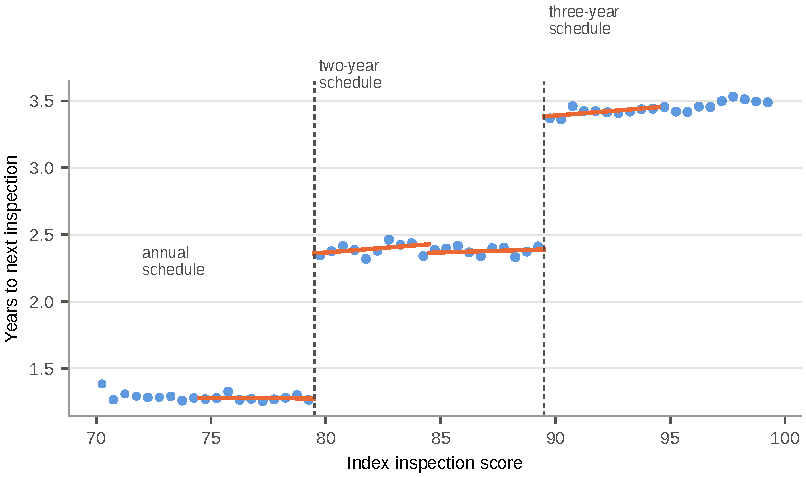
\includegraphics[width=0.82\textwidth]{figs/first_stage.pdf}
\caption{First stage. Mean years to the next inspection by index score, in half-point bins (marker size proportional to count), with local linear fits within five points of each cutoff. Dashed lines mark the cutoffs at 79.5 and 89.5.}\label{fig:fs}
\end{figure*}

\subsection{Validity}
Table~\ref{tab:validity} reports the validity checks. No predetermined variable jumps at either cutoff. At 90 neither density test detects sorting. At 80 the two density tests disagree: the binned estimator gives $\hat\rho=\densLrEighty$ ($z=\densZEighty$) while \texttt{rddensity} rejects continuity ($t=\rddTEighty$, $p=\rddPEighty$). The plan did not specify which test governs its decision rule. We apply the stricter reading, so the donut estimate is the headline at 80. Fig.~\ref{fig:density} shows the distribution of index scores.

The share of index inspections with a next inspection observed falls by \secAttrEighty{} percentage points at 80 and \secAttrNinety{} at 90. Of index inspections without a next inspection, \absentLater\% belong to properties absent from every later HUD file, consistent with exit from the portfolio during the extra year.

\begin{table}[t]
\caption{Validity checks at the cutoffs}\label{tab:validity}
\centering\scriptsize\setlength{\tabcolsep}{3pt}
\resizebox{\columnwidth}{!}{\begin{tabular}{lrrrr}
\toprule
& \multicolumn{2}{c}{80 cutoff} & \multicolumn{2}{c}{90 cutoff} \\
\cmidrule(lr){2-3}\cmidrule(lr){4-5}
Outcome & Jump (SE) & $p$ & Jump (SE) & $p$ \\
\midrule
Previous score & $-$0.63 (0.72) & 0.38 & +0.57 (0.61) & 0.35 \\
Inspection sequence number & $-$0.04 (0.04) & 0.33 & $-$0.01 (0.03) & 0.83 \\
Index year & $-$0.03 (0.05) & 0.64 & +0.04 (0.05) & 0.39 \\
Index month & +0.13 (0.13) & 0.31 & +0.06 (0.11) & 0.58 \\
Next inspection listed (attrition) & $-$0.035 (0.010) & 0.000 & $-$0.040 (0.010) & 0.000 \\
Density, binned log ratio & +0.056 (0.037) & 0.127 & +0.001 (0.031) & 0.968 \\
Density, \texttt{rddensity} $t$ & +2.34 & 0.019 & $-$0.42 & 0.674 \\
\bottomrule
\end{tabular}
}
\tabnote{Rows 1--5: jump at the cutoff from the primary specification ($h=5$), standard errors clustered by property. Density rows: binned log-ratio estimator (bandwidth 6) and the local polynomial test of~\cite{cattaneo2020}.}
\end{table}

\begin{figure}[t]
\centering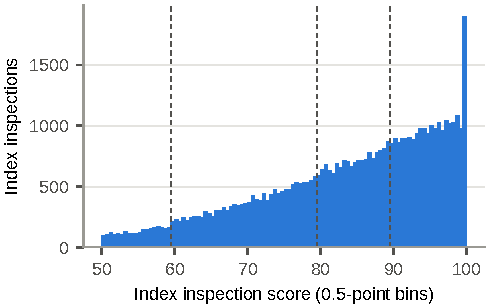
\includegraphics[width=\columnwidth]{figs/density_col.pdf}
\caption{Distribution of index inspection scores, 2001--2005, in half-point bins. Dashed lines mark 59.5, 79.5 and 89.5.}\label{fig:density}
\end{figure}

\subsection{Main Results}
Fig.~\ref{fig:rf} plots the next score against the index score, and Table~\ref{tab:rd} reports the estimates. The registered primary estimate is \jumpEighty{} points at 80 (standard error \seEighty; 95\% CI \ciLoEighty{} to \ciHiEighty; $p=\pEighty$, Holm $p=\pHolmEighty$) and \jumpNinety{} at 90 (\seNinety; \ciLoNinety{} to \ciHiNinety; $p=\pNinety$, Holm $p=\pHolmNinety$). Neither null hypothesis is rejected. Per additional year between inspections, the fuzzy estimates are \waldEighty{} (\waldSeEighty) and \waldNinety{} (\waldSeNinety) points.

Under the registered decision rule, the headline at 80 is the donut estimate: \robDonutOneEighty{} points (\robDonutOneSeEighty; 95\% CI \robDonutOneCiLoEighty{} to \robDonutOneCiHiEighty; $p=\robDonutOnePEighty$). It is larger in magnitude and less precise than the primary estimate, and also not significant.

\begin{figure*}[t]
\centering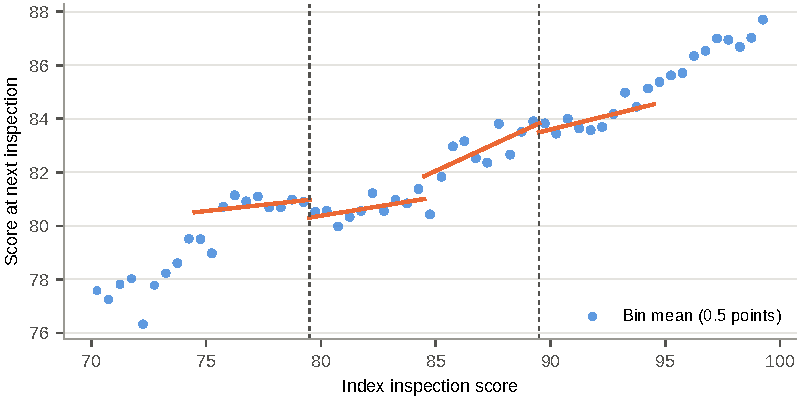
\includegraphics[width=0.82\textwidth]{figs/reduced_form.pdf}
\caption{Reduced form. Mean score at the next inspection by index score, in half-point bins, with local linear fits within five points of each cutoff.}\label{fig:rf}
\end{figure*}

\begin{table*}[t]
\caption{Effect of crossing a schedule cutoff on the next inspection score}\label{tab:rd}
\centering\footnotesize
\begin{tabular}{lcc}
\toprule
& 80 cutoff & 90 cutoff \\
\midrule
Primary: local linear, $h=5$ & $-$0.66 & $-$0.33 \\
 & (0.58) & (0.46) \\
Bandwidth $h=3$ & $-$0.25 & $-$0.18 \\
 & (0.75) & (0.58) \\
Bandwidth $h=8$ & $-$1.37 & $-$0.72 \\
 & (0.46) & (0.37) \\
Local quadratic, $h=8$ & $-$0.13 & $-$0.21 \\
 & (0.67) & (0.53) \\
Donut, $|x-c|\geq0.5$ & $-$0.96 & $-$0.32 \\
 & (0.73) & (0.59) \\
Donut, $|x-c|\geq1$ & $-$1.56 & $-$0.22 \\
 & (0.96) & (0.78) \\
Excluding first listed inspection & $-$0.62 & $-$0.65 \\
 & (0.72) & (0.63) \\
\texttt{rdrobust}, bias-corrected & $-$0.10 & $-$0.02 \\
\quad robust 95\% CI; MSE-optimal $h$ & [$-$1.62, 1.42]; 3.69 & [$-$1.28, 1.25]; 3.36 \\
Trimming bounds (attrition) & [$-$2.28, +0.10] & [$-$1.88, +0.40] \\
\midrule
Observations, primary & 10,993 & 15,183 \\
First stage (years), primary & 1.08 (0.024) & 0.99 (0.022) \\
\bottomrule
\end{tabular}

\tabnote{\centering Jump in the next score (points) at the cutoff; standard errors clustered by property in parentheses. Triangular kernel and local linear fit unless stated. \texttt{rdrobust}: MSE-optimal bandwidth with robust bias-corrected inference~\cite{calonico2014}. Trimming bounds follow~\cite{lee2009}.}
\end{table*}

\subsection{Robustness}
Fig.~\ref{fig:rob} collects the registered robustness checks. With MSE-optimal bandwidths of \rdrHEighty{} and \rdrHNinety{} points, the bias-corrected estimates are \rdrBcEighty{} (robust 95\% CI \rdrLoEighty{} to \rdrHiEighty) and \rdrBcNinety{} (\rdrLoNinety{} to \rdrHiNinety). The trimming bounds are [\leeLoEighty, \leeHiEighty] at 80 and [\leeLoNinety, \leeHiNinety] at 90, both including zero. The placebo cutoffs show no jump (Table~\ref{tab:placebo}).

Linear fits over a wider bandwidth of eight points give larger, significant estimates (\robHEightEighty{} at 80, $p=\robHEightPEighty$; \robHEightNinety{} at 90, $p=\robHEightPNinety$). Allowing curvature at the same bandwidth removes them (\robQuadEighty{} and \robQuadNinety). Fig.~\ref{fig:rf} shows the mechanism: the relation between index and next score is concave within each schedule band, so a straight line fitted over eight points misplaces the limit at the cutoff. We read the wide-bandwidth linear estimates as specification error; the data-driven bandwidths, which trade off this bias against variance, are narrower than five points.

\begin{figure*}[t]
\centering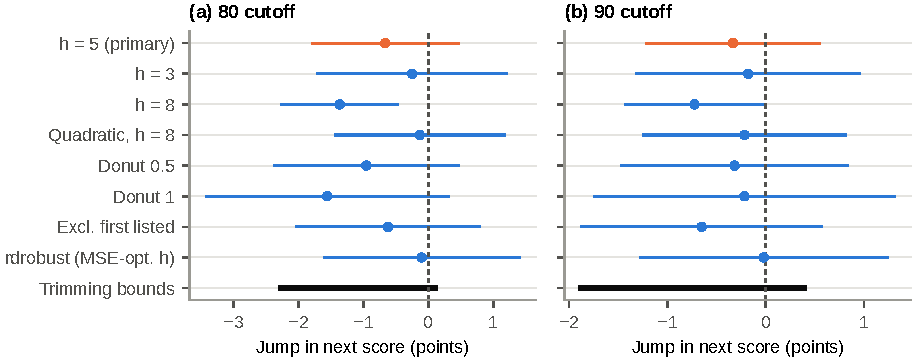
\includegraphics[width=0.82\textwidth]{figs/robustness.pdf}
\caption{Estimates across registered specifications with 95\% confidence intervals. The primary estimate is highlighted; the black bar is the interval between the trimming bounds for differential attrition.}\label{fig:rob}
\end{figure*}

\begin{table}[t]
\caption{Placebo cutoffs ($h=4$)}\label{tab:placebo}
\centering\scriptsize
\begin{tabular}{lrrr}
\toprule
Placebo cutoff & Jump (SE) & $p$ & $n$ \\
\midrule
74.5 & $-$0.16 (0.72) & 0.82 & 7,064 \\
84.5 & $-$0.27 (0.60) & 0.65 & 10,394 \\
94.5 & +0.02 (0.47) & 0.97 & 13,833 \\
\bottomrule
\end{tabular}

\end{table}

\subsection{Secondary Outcomes}
Table~\ref{tab:secondary} reports the secondary outcomes. The probability that the next inspection fails changes by \secFailEighty{} percentage points at 80 ($p=\secFailPEighty$) and \secFailNinety{} at 90 ($p=\secFailPNinety$). The fixed-horizon score, which compares properties at roughly the same elapsed time, changes by \secFixedEighty{} at 80 and \secFixedNinety{} at 90. None is significant, though the failure estimate at 80 is positive with $p$ close to 0.06.

\begin{table}[t]
\caption{Secondary outcomes ($h=5$)}\label{tab:secondary}
\centering\scriptsize\setlength{\tabcolsep}{2.5pt}
\resizebox{\columnwidth}{!}{\begin{tabular}{lrrrrrr}
\toprule
& \multicolumn{3}{c}{80 cutoff} & \multicolumn{3}{c}{90 cutoff} \\
\cmidrule(lr){2-4}\cmidrule(lr){5-7}
Outcome & Jump (SE) & $p$ & $n$ & Jump (SE) & $p$ & $n$ \\
\midrule
Next inspection fails (pp) & +2.1 (1.1) & 0.063 & 10,993 & +0.5 (0.8) & 0.535 & 15,183 \\
Fixed-horizon score (points) & +0.50 (0.61) & 0.412 & 10,595 & $-$0.36 (0.46) & 0.425 & 15,170 \\
Fuzzy: points per additional year & $-$0.61 (0.54) & 0.252 & 10,993 & $-$0.33 (0.46) & 0.467 & 15,183 \\
\bottomrule
\end{tabular}
}
\tabnote{Standard errors clustered by property in parentheses. Fixed-horizon score: score at the first inspection at least 21 months after the index inspection. Fuzzy: reduced form divided by the first-stage jump in years.}
\end{table}

\section{Is the Mass at 59 Mechanical?}\label{sec:bunching}
Fig.~\ref{fig:bunch} shows NSPIRE scores and the fitted counterfactual. The excess at 59 is $\hat B=\excMf$ (standard error \excSeMf) for multifamily and \excPh{} (\excSePh) for public housing, \excRatioMf{} and \excRatioPh{} times the counterfactual count. The missing mass in $[60,70]$ is $\hat M=\misMf$ (\misSeMf) and \misPh{} (\misSePh). The registered test statistic is $\hat\Delta=\difMf$ (\difSeMf; $z=\difZMf$, Holm $p=\difPHolmMf$) for multifamily and \difPh{} (\difSePh; $z=\difZPh$, Holm $p=\difPHolmPh$) for public housing. The excess at 59 is fully accounted for by the deficit above it.

\begin{figure*}[t]
\centering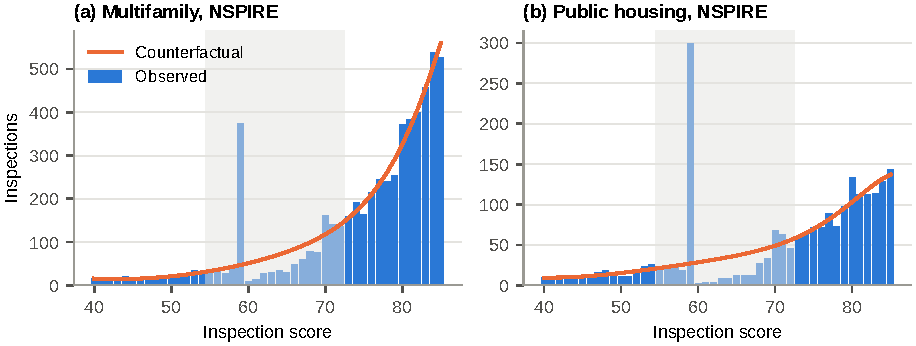
\includegraphics[width=0.82\textwidth]{figs/bunching.pdf}
\caption{NSPIRE scores (bars) and the counterfactual distribution (line), a fifth-order polynomial in log counts fitted to scores 40--85 outside the shaded window 55--72.}\label{fig:bunch}
\end{figure*}

\begin{table*}[t]
\caption{Excess mass at 59 and missing mass in 60--70}\label{tab:bunching}
\centering\footnotesize
\begin{tabular}{llcrrr}
\toprule
Sample & Order & Excluded & Excess at 59 & Missing in 60--70 & Difference \\
\midrule
Multifamily & 5 & 55--72 & 328 (20) & 316 (103) & 12 (112) \\
 & 4 & 55--72 & 328 (21) & 370 (157) & -42 (167) \\
 & 6 & 55--72 & 322 (27) & 428 (356) & -106 (375) \\
 & 5 & 53--74 & 336 (23) & 139 (151) & 197 (164) \\
 & 5 & 56--71 & 327 (21) & 318 (86) & 9 (94) \\
\quad UPCS 2013--19 (comparison) & 5 & 55--72 & -22 (23) & -1,182 (248) & 1,160 (263) \\
\midrule
Public housing & 5 & 55--72 & 273 (19) & 223 (63) & 50 (70) \\
 & 4 & 55--72 & 273 (18) & 250 (88) & 23 (94) \\
 & 6 & 55--72 & 271 (20) & 251 (229) & 20 (241) \\
 & 5 & 53--74 & 282 (18) & 111 (79) & 171 (86) \\
 & 5 & 56--71 & 275 (17) & 179 (50) & 97 (55) \\
\quad UPCS 2013--19 (comparison) & 5 & 55--72 & 13 (16) & -451 (136) & 464 (146) \\
\bottomrule
\end{tabular}

\tabnote{\centering Counts of inspections relative to the counterfactual; bootstrap standard errors (500 Poisson resamples) in parentheses. The first row for each program is the registered specification. UPCS rows are a comparison in which no unit-threshold rule operates.}
\end{table*}

Table~\ref{tab:bunching} shows sensitivity to the counterfactual. Polynomial order and a narrower window leave the result unchanged. A wider window (53 to 74) leaves less data to anchor the fit near the threshold and yields a larger positive $\hat\Delta$, significant at the 5\% level for public housing. The UPCS comparison finds no excess at 59 (\upcsExcMf{} and \upcsExcPh), as expected without the rule, but a nonzero $\hat\Delta$, because under UPCS the range 60 to 70 holds \emph{more} inspections than the counterfactual. That surplus reflects sorting toward the passing score.

\subsection{Sorting Under UPCS}
Table~\ref{tab:thresholds} compares observed and counterfactual counts around each threshold for UPCS inspections from 2013 to 2019. Multifamily scores show a deficit just below 60 (\thrMfSixtyBelow\%) and a surplus just above (\thrMfSixtyAbove\%), and the same pattern at 80 (\thrMfEightyBelow\% and \thrMfEightyAbove\%). Public housing shows it at 80 and, weakly, at 60. At 90 there is no clear asymmetry. In the 2001--2005 history sample the density of index scores is about \histDensPct\% higher just above 59.5 than just below ($z=\histDensZ$). Movement from just below a threshold to just above it is what the technical-review rule rewards. Under NSPIRE the range just above 60 is depleted rather than inflated, because the unit threshold moves properties in the opposite direction.

\begin{table*}[t]
\caption{Observed and counterfactual counts around thresholds, UPCS 2013--2019}\label{tab:thresholds}
\centering\footnotesize
\begin{tabular}{lrrrrrrr}
\toprule
& & \multicolumn{3}{c}{Two scores below} & \multicolumn{3}{c}{Two scores at or above} \\
\cmidrule(lr){3-5}\cmidrule(lr){6-8}
Program & Threshold & Observed & Counterf. & Diff. (\%) & Observed & Counterf. & Diff. (\%) \\
\midrule
Multifamily & 60 & 473 & 671 & $-$30 & 942 & 804 & 17 \\
 & 80 & 2,440 & 2,737 & $-$11 & 3,343 & 3,106 & 8 \\
 & 90 & 4,841 & 4,564 & 6 & 5,202 & 4,949 & 5 \\
Public housing & 60 & 266 & 285 & $-$7 & 347 & 323 & 7 \\
 & 80 & 736 & 827 & $-$11 & 999 & 908 & 10 \\
 & 90 & 1,226 & 1,245 & $-$1 & 1,444 & 1,299 & 11 \\
\bottomrule
\end{tabular}

\tabnote{\centering Counterfactual from a quadratic fitted to integer scores $c-10$ to $c+9$ excluding $c-2$ to $c+1$. Registered as descriptive; no standard errors were pre-specified.}
\end{table*}

\section{The October 2026 Change}\label{sec:h3}
The registered hypothesis H3 is that, for the same properties, NSPIRE inspections on or after 1 October 2026 have lower scores, a higher share below 60 and a higher share at exactly 59. The analysis will run once, on the first HUD file whose inspections reach at least 31 March 2027, estimating
\begin{equation}
y_{it}=\alpha_i+\delta_{g(i),\text{yr}(t)}+\beta\,\mathbb 1[t\ge\text{2026-10-01}]+\varepsilon_{it}
\end{equation}
for each outcome, with property effects $\alpha_i$, program-by-year effects $\delta$, standard errors clustered by property and Holm's correction across the three outcomes. The plan states one limitation in advance: properties reinspected soon after the change are disproportionately those that scored low before, which biases the comparison toward improvement, and the property effects do not remove this.

\section{Discussion}\label{sec:discussion}
\runhead{Interpreting the null.} Near the 80 and 90 thresholds, being assigned an extra year between inspections did not measurably lower the score at the next inspection. Three explanations fit this result. Conditions may change slowly enough that an extra year matters little for properties scoring between about 75 and 95. Owners may maintain to a standard set by other pressures, such as lenders, local codes and residents, rather than by the federal inspection calendar. Or reduced monitoring may lower effort while the anticipated inspection still disciplines it, with a net effect too small to detect. The design cannot separate these explanations. The primary estimates rule out declines larger than \ciLoEighty{} points at 80 and \ciLoNinety{} at 90. The donut estimate at 80 is less precise and cannot exclude declines of up to \robDonutOneCiLoEighty{} points.

\runhead{Implications for inspection design.} A risk-based schedule is justified if the entities it inspects less often do not deteriorate faster. Near HUD's thresholds, under UPCS and for multifamily properties, we find no evidence that they did. This does not show that inspection is ineffective, since every property in the sample was inspected, nor that less frequent inspection is harmless for properties far from the thresholds.

\runhead{The score as a measure.} Under UPCS, scores just below the passing mark and the 80 cutoff are under-represented, consistent with successful challenges. Under NSPIRE, the excess at 59 is produced by a rule, so a score of 59 is a category (``failed on unit conditions'') rather than a point on a continuous scale. Studies that treat scores near 60 as continuous, including regression discontinuity designs at the passing score, need to account for both features.

\section{Limitations}\label{sec:limits}
\begin{enumerate}
\item \textbf{Local estimates.} The results apply to multifamily properties scoring near 80 and 90 between 2001 and 2005, under UPCS. They do not extend directly to low-scoring properties, public housing, or NSPIRE.
\item \textbf{Outcome timing.} The reduced form mixes reduced monitoring with an extra year of elapsed time. The fixed-horizon outcome addresses this only approximately.
\item \textbf{Selection on follow-up.} Follow-up is less likely above each cutoff. The trimming bounds are wide relative to the point estimates.
\item \textbf{Sorting at 80.} One of two density tests rejects at 80, and the donut estimate that the plan makes the headline there is imprecise.
\item \textbf{The outcome is HUD's score.} It measures what the protocol records and is subject to inspector variation~\cite{gao2019}.
\item \textbf{The bunching test is indirect.} Unit deductions are not published, and the result is sensitive to a wider excluded window.
\item \textbf{Completeness of the history file.} It is treated as a complete listing of 2000--2009 inspections, which public sources cannot verify.
\end{enumerate}

\section{Conclusion}
HUD's inspection schedule assigns substantially different monitoring intensity to properties in nearly identical condition. A pre-registered regression discontinuity analysis finds no measurable effect of an extra year between inspections on the next score near the 80 and 90 thresholds. The excess of NSPIRE scores at exactly 59 satisfies the restriction implied by the unit-threshold rule, while the earlier protocol shows sorting toward passing. The effect of scoring NSPIRE affirmative requirements will be estimated, as registered, when the data exist.

\section*{Pre-Registration and Deviations}
The plan was registered at \url{https://osf.io/ab2es} before any outcome contrast was computed. Deviations:
(1)~The plan named two density tests without specifying which governs its decision rule; they disagree at 80, and we applied the stricter reading (donut headline at 80) while reporting the primary estimate alongside.
(2)~\texttt{rdrobust}~2.1.1 and \texttt{rddensity}~3.0 were installed from PyPI wheels with verified hashes. Their plotting dependency was replaced by an import-only stub because no plots from those packages are used. \texttt{rdrobust} detects mass points in the running variable and applies its default adjustment.
(3)~H3 has not been run because the data do not yet exist, as anticipated.
There are no other departures.

\section*{Data and Code Availability}
Data: AHCP v1.0, \url{https://doi.org/10.5281/zenodo.23200319}. Code, registered plan, design checks, outputs and the scripts that generate every number, table and figure in this article: \url{https://github.com/AYISHATUAMEEN/inspection-rd}.

\section*{Acknowledgment}
\emph{Use of AI tools:} code, data processing, figures and a draft of this article were prepared with the assistance of Claude (Anthropic). The author designed and registered the study, made the analytic decisions, verified the results and is responsible for all content. The author declares no competing interests.

\begin{thebibliography}{99}\footnotesize\setlength{\itemsep}{0pt}\setlength{\parskip}{0pt}
\bibitem{gray2011} W. B. Gray and J. P. Shimshack, ``The effectiveness of environmental monitoring and enforcement: a review of the empirical evidence,'' \emph{Rev. Environ. Econ. Policy}, vol. 5, no. 1, pp. 3--24, 2011.
\bibitem{shimshack2014} J. P. Shimshack, ``The economics of environmental monitoring and enforcement,'' \emph{Annu. Rev. Resour. Econ.}, vol. 6, pp. 339--360, 2014.
\bibitem{fr2000} U.S. Department of Housing and Urban Development, ``Uniform physical condition standards and physical inspection requirements for certain HUD housing; administrative process for assessment of insured and assisted properties,'' final rule, 65 Fed. Reg. 77230, Dec. 8, 2000.
\bibitem{osfplan} A. Ameen, ``Do inspection thresholds improve housing conditions? Pre-analysis plan,'' OSF Registries, 2026. [Online]. Available: \url{https://osf.io/ab2es}
\bibitem{ahcp} A. Ameen, ``Assisted Housing Condition Panel (AHCP) v1.0,'' Zenodo, dataset, 2026, doi: 10.5281/zenodo.23200319.
\bibitem{ameen2026} A. Ameen, ``The Assisted Housing Condition Panel: reconstructing inspection histories for HUD-assisted housing from overwritten public score files,'' working paper, 2026.
\bibitem{nspirescoring} U.S. Department of Housing and Urban Development, ``National Standards for the Physical Inspection of Real Estate and associated protocols, scoring notice,'' 88 Fed. Reg. 43371, July 7, 2023.
\bibitem{levine2012} D. I. Levine, M. W. Toffel, and M. S. Johnson, ``Randomized government safety inspections reduce worker injuries with no detectable job loss,'' \emph{Science}, vol. 336, no. 6083, pp. 907--911, 2012.
\bibitem{jin2003} G. Z. Jin and P. Leslie, ``The effect of information on product quality: evidence from restaurant hygiene grade cards,'' \emph{Quart. J. Econ.}, vol. 118, no. 2, pp. 409--451, 2003.
\bibitem{duflo2013} E. Duflo, M. Greenstone, R. Pande, and N. Ryan, ``Truth-telling by third-party auditors and the response of polluting firms: experimental evidence from India,'' \emph{Quart. J. Econ.}, vol. 128, no. 4, pp. 1499--1545, 2013.
\bibitem{lee2010} D. S. Lee and T. Lemieux, ``Regression discontinuity designs in economics,'' \emph{J. Econ. Lit.}, vol. 48, no. 2, pp. 281--355, 2010.
\bibitem{mccrary2008} J. McCrary, ``Manipulation of the running variable in the regression discontinuity design: a density test,'' \emph{J. Econometrics}, vol. 142, no. 2, pp. 698--714, 2008.
\bibitem{cattaneo2020} M. D. Cattaneo, M. Jansson, and X. Ma, ``Simple local polynomial density estimators,'' \emph{J. Amer. Statist. Assoc.}, vol. 115, no. 531, pp. 1449--1455, 2020.
\bibitem{calonico2014} S. Calonico, M. D. Cattaneo, and R. Titiunik, ``Robust nonparametric confidence intervals for regression-discontinuity designs,'' \emph{Econometrica}, vol. 82, no. 6, pp. 2295--2326, 2014.
\bibitem{lee2009} D. S. Lee, ``Training, wages, and sample selection: estimating sharp bounds on treatment effects,'' \emph{Rev. Econ. Stud.}, vol. 76, no. 3, pp. 1071--1102, 2009.
\bibitem{kleven2016} H. J. Kleven, ``Bunching,'' \emph{Annu. Rev. Econ.}, vol. 8, pp. 435--464, 2016.
\bibitem{gao2019} U.S. Government Accountability Office, ``Real Estate Assessment Center: HUD should improve physical inspection process and oversight of inspectors,'' GAO-19-254, Mar. 2019.
\bibitem{nspirerule} U.S. Department of Housing and Urban Development, ``Economic Growth Regulatory Relief and Consumer Protection Act: implementation of National Standards for the Physical Inspection of Real Estate (NSPIRE),'' final rule, 88 Fed. Reg. 30442, May 11, 2023.
\bibitem{cfr5705} U.S. Department of Housing and Urban Development, ``Physical condition standards and inspection requirements: timing of inspections,'' 24 C.F.R. \S~5.705(c).
\bibitem{fr2026} U.S. Department of Housing and Urban Development, ``National Standards for the Physical Inspection of Real Estate: scoring notice; request for public comment,'' FR Doc. 2026-19881, Sep. 29, 2026.
\bibitem{holm1979} S. Holm, ``A simple sequentially rejective multiple test procedure,'' \emph{Scand. J. Statist.}, vol. 6, no. 2, pp. 65--70, 1979.
\end{thebibliography}

\clearpage
\onecolumn
\begin{center}\textsc{Appendix: Estimator Validation and Algorithms}\end{center}

\appsection{A}{Validation of the Estimators on Synthetic Data}
Before registration, the estimators in the replication package were tested on synthetic data with known answers (\texttt{code/00\_simulation\_tests.py}). The sharp and fuzzy RD tests use 400 replications with a clustered error structure; the density tests use 400 replications with and without a relocation of 25\% of the mass just below the cutoff to just above it; and the bunching tests use 100 replications that move half of the mass in $[60,70]$ to 59. Table~\ref{tab:sim} lists the results; \simAllPass{} criteria were met. As a further check, the project's local linear estimator reproduces the conventional estimate of \texttt{rdrobust} at a fixed bandwidth on synthetic data.

\begin{table}[h]
\caption{Estimator validation on synthetic data}\label{tab:sim}
\centering\footnotesize
\begin{tabular}{lll}
\toprule
Check & Result & Criterion met \\
\midrule
Sharp RD unbiased & mean 2.020 (true 2.0) & yes \\
Sharp RD coverage & 0.965 & yes \\
Fuzzy RD unbiased & median $-$1.498 (true $-$1.5) & yes \\
Fuzzy RD coverage & 0.973 & yes \\
Density test size & 0.048 & yes \\
Density test power & 1.000 & yes \\
Bunching excess recovered & mean relative error $-$0.003 & yes \\
Bunching excess equals missing under pure relocation & 25 (se 156) & yes \\
\bottomrule
\end{tabular}

\end{table}

\appsection{B}{Algorithms}
\runhead{Sample construction.} (1)~Select multifamily inspections from the 2011 history file. (2)~Sort each property's inspections by date; attach the next inspection's date and score and the previous inspection's score. (3)~Keep index inspections dated 8 January 2001 to 31 December 2005. (4)~The fixed-horizon outcome is the score at the first listed inspection at least 21 months after the index date.

\runhead{Trimming bounds.} (1)~Estimate the jump $\hat\delta$ in $R_i$ and the below-cutoff limit $\hat r^-$; set $q=\max(\hat\delta,0)/\hat r^-$. (2)~Among observed outcomes with $c-h\le X_i<c$, compute the $q$ and $1-q$ quantiles. (3)~Drop the observations above the $1-q$ quantile and re-estimate to obtain the upper bound; drop those below the $q$ quantile for the lower bound.

\runhead{Bunching test.} (1)~Count inspections at each integer score from 40 to 85. (2)~Fit a polynomial of the stated order to $\log\max(n_s,0.5)$ outside the excluded window. (3)~Compute $\hat B$, $\hat M$ and $\hat\Delta$. (4)~Repeat on 500 Poisson resamples of the counts and report the standard deviations as standard errors.

\end{document}
